%qqqqqqqqqqqqqqqqqqqqqqqqqqqqqqqqqqqqqqqqqqqqqqqqqqqqqqqqqqqqqqqqqqqqqqqqq
%Quote
\begin{savequote}[50mm]
%‘‘El cosmos es todo lo que es, todo lo que fue y todo lo que será. Nuestras 
%más ligeras contemplaciones del cosmos nos hacen estremecer: Sentimos como 
%un cosquilleo nos llena los nervios, una voz muda, una ligera sensación como
%de un recuerdo lejano o como si cayéramos desde gran altura. Sabemos que nos
%aproximamos al más grande de los misterios.’’
%\qauthor{Carl Sagan}
\end{savequote}
%qqqqqqqqqqqqqqqqqqqqqqqqqqqqqqqqqqqqqqqqqqqqqqqqqqqqqqqqqqqqqqqqqqqqqqqqq

%*****************************************************
\chapter{Algoritmo y modelación}
\label{cha:Modelo de Spin}
%*****************************************************
%El desarrollo de modelos computacionales permiten reproducir sucesos que escapan a acontecer de una vida humana. Es por eso la importancia de los modelos

En la búsqueda de poder conocer como se pueden alinear los SMBH en AGNs con su entorno, se hace necesario el uso de modelos computacionales que sean capaces de reproducir lo fenómenos físicos que ocurren en el universo. Para nuestro propósito se hace uso de una serie de simulaciones cosmológicas auto-consistentes, que son capaces de simular la evolución de los espines de los SMBHs, ratas de acreción de BHs, feadback de BHs y propiedades de galaxias donde se hospedan los BHs. La simulación que se va usar para tal propósito es el código de Magneto-hidrodinámica para N-cuerpos AREPO \cite{springel2010}, que es capaz de reproducir mallas que cambian de forma, moviendosen con el fluido, y hace seguimiento a las propiedades del gas. Sin embargo, también se hace uso de otros métodos computacionales que permiten conocer cómo se distribuye la materia en el universo o mejor aun, permiten hacer una clasificación y estructuración del mismo. El método que se usa para la clasificación de las estructuras en el universo es el T-web \cite{hahn2007}, que es capaz de categorizar las regiones del universo usando un modelo de sistemas dinámicos. Para el modelo de detección de sub estructuras, que permite localizar zonas de sobre densidad, que indican la presencia de un halo de materia oscura, grupo o cúmulo  de galaxias. 

%*****************************************************
\section{Código Arepo}
\label{sec: codigo arepo}
%***********************************************

%El código {\textsc{Arepo}} es una simulación cosmológica, que pretende diseñar una nueva forma de hacer simulaciones hidrodinámicas que son capaces reproducir la dinámica del universo, evolución estelar, formación de estructuras y evolución de parámetros en las galaxia. Este modelo hidrodinámico tiene como objetivo mejorar dos códigos muy usados en la simulaciones de formación y evolución: Mallado de Euleriano y la técnica  hidrodinámica de suavizado de partículas Lagrangiana (SPH). 

En la astrofísica se hace necesario poder contrastar los modelos teóricos con lo observacional. Es por eso que se hace uso de los modelos computacionales que al usar los modelos teóricos pueda obtener como resultado lo observacional. Una forma de poder reproducir lo que ocurre en el universo se considera la dinámica de fluidos haciendo uso de los modelos hidrodinámicos, los modelos más sobresalientes en este ámbito son: SPH \cite{monaghan1992} y hidrodinámica Euleriana basada en mallas \cite{stone2008} con refinamiento adaptativo de las mallas (AMR). A pesar de ser los modelos más usados en la hidrodinámica presentan una serie de falencias:

- SPH es pobre en resolución,  ofrecen precesión de bajo orden para el tratamiento de discontinuidades de contacto, y en algunos casos suprime inestabilidades de los fluidos

- Mallas Eulerianas no producen invariantes galileanos, implicando que los resultados son sensibles para grandes cambios en velocidades de volumen.\\

En busqueda de poder mejorar las falencias de las simulaciones mencionadas y además tomar lo mejor de cada una, el código  {\it{Arepo}} toma lo mejor de cada simulación y mejora las falelcias de cada una. En general el código {\it{Arepo}} \cite{springel2010} introduce una nueva forma de modelación hidrodinámica continua en mallas dinámicas. Lo que se va argumentar a continuación esta basado en \cite{springel2010}:

La precisión del modelo viene determinado mayormente por su nueva forma de diseñar las mallas (grid). Se define la malla bajo la teselación de Voronoi de un conjunto de puntos que se distribuyen espacialmente y se les permite mover libremente. 

El método de Voronoi es el método de interpolación más simple, que se basa en la distancia euclidea. Permite crear celdas de tal forma que la región encerrada esta lo más cerca posible a sus celdas vecinas. Los polígonos se diseñan al unir los puntos entre si, trazando luego una mediatriz entre los segmentos de unión. La intersección de las mediatrices dan como resultado los polígonos y por lo tanto la malla (ver figura \ref{fig: voronoi}). Cada celda en la malla lleva consigo variables de fluido que se conservan (masa, momentum y energía total).
%
\begin{center}
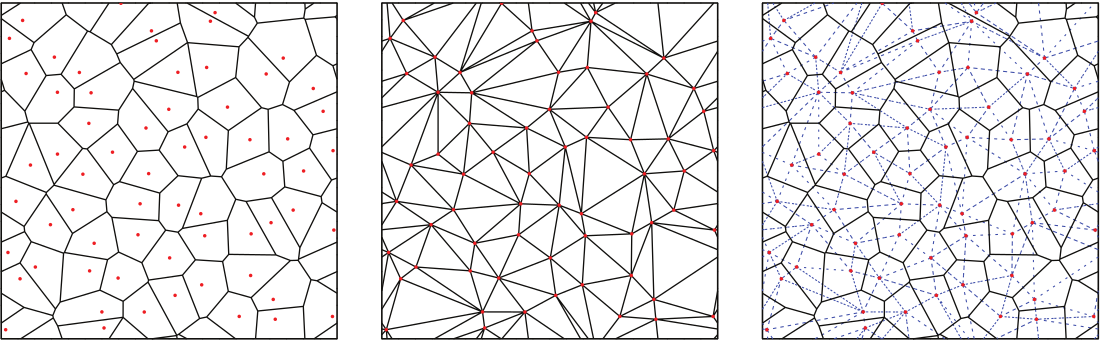
\includegraphics[scale=.35]{./figures/5_Algoritmo_Modelacion/voronoi.png}
\figcaption{\emph{Representación gráfica de la teselación de Voronoi. En esta gráfica se puede ver la doble topología del digrama de Voronoi, pues es equivalente topológicamente a la teselación de Delaunay.}}\label{fig: voronoi}
\end{center}
%
La importancia de la simulación Voronoid, es que permite que los puntos en la malla se muevan con el fluido a la velocidad del fluido, esto permite que a medida que trascurren los pasos numéricos, se actualice la información del fluido en la celda. Este método permite solucionar el problema de no invariabilidad galileana que emergía del método de la malla de Euler. Al solucionar esto se impide la alta sensibilidad en el cambio de las velocidades, haciendo que la dinámica del sistema sea consistente, por ende se obtengan valores no sesgados para la alineación de los BHs en cada celda y del momentum angular del gas que circula alrededor del BH. 

Este método permite que en las regiones donde hay una sobre densidad de materia, se generan una mayor cantidad de celdas, mientras que en un región donde la sobre densidad es pequeña el número de celdas, permitiendo modelar de forma más precisa la dinámica y acreción de materia en los BHs.

El objetivo principal de la simulación es poder solucionar las ecuaciones del fluido, para ello hace uso de las ecuaciones de Euler, que son leyes de la conservación de la masa, energía y momentum, que toma la forma de un sistema de ecuaciones diferenciales parciales hiperbólicas. \cite{springel2010} reescribe de forma compacta las ecuaciones de conservación o de fluido de la siguiente forma:

Se introduce el vector de estado    
\begin{align}
    \vec{\bf{U}}= \begin{pmatrix} \rho \\ \rho\vec{v} \\ \rho e \end{pmatrix} = 
    \begin{pmatrix} \rho \\ \rho\vec{v} \\ \rho u+\frac{1}{2}\rho\vec{v}^{2} \end{pmatrix}\,,
\end{align}
donde $\rho$ es la densidad del fluido, $\vec{v}$ es el campo de velocidad y $e=u+ \vec{v}^{2}/2$ es la energía por unidad de masa. el parámetro $u$ indica la energía térmica por unidad de masa. Las cantidades del fluido son dependientes del espacio y del tiempo $\vec{\bf{U}}(\vec{\bf{x}},t)$, se define además la función de flujo

\begin{align}
    \vec{\bf{F}}(\vec{\bf{U}})=
    \begin{pmatrix} \rho\vec{v} \\ \rho\vec{v}\vec{v}^{T}+ P \\ (\rho e + P)\vec{v} \end{pmatrix}\,,
\end{align}
donde $P$ es la ecuación de estado queda la presión del fluido. Es por tanto que la ecuación de Euler se puede escribir de forma compacta como 
\begin{align}
    \frac{\partial\vec{\bf{U}}}{\partial t} + \vec{\nabla}\cdot \vec{\bf{F}}\,.
\end{align}

En el código de {\it{Arepo}} se considera una discretización del fluido como un conjunto de volúmenes finitos, donde cada celda se identifica bajo el uso de un contador "$i$". Cada celda contiene la información de la masa $m_{i}$, momentum $p_{i}$ y la energía $E_{i}$. %
\begin{align}
    {\bf{Q}_{i}} = \begin{pmatrix} m_{i} \\ p_{i} \\ E_{i} \end{pmatrix} = \int_{V_{i}} \vec{\bf{U}}d\vec{\bf{V}}\,.
\end{align}
%
Usando la ecuación de Euler, es posible calcular la razón de cambio de ${\bf{Q}_{i}}$ en el tiempo, al usar el teorema de Gauss
%\
\begin{align}
    \frac{d{\bf{Q_{i}}}}{dt} = -\int_{\partial V_{i}}[\vec{\bf{F}}(\vec{\bf{U}})-\vec{\bf{U}}\vec{\bf{w}}^{T}]d\vec{\bf{n}}\,,
\end{align}
donde $\vec{\bf{w}}$ es la velocidad particular de cada partícula y $\vec{\bf{n}}$ es el vector normal a la superficie.

El nuevo esquema presentado por \cite{springel2010} indica cuales fueron los pasos (algoritmia) que sigue el código. Parte del estado del fluido para cada celda ${\bf{Q_{i}}}$ y al hacerlo evolucionar es capaz de dar los resultados no invarianza galileana y buena resolución en la simulaciones. 

%*****************************************************
\section{Caracterización del entorno}
\label{sec: Caracterizacion entorno}
%*****************************************************

Al recordar lo mencionado en (\ref{sec: Estructure_Formation}), es posible decir que las simulaciones computacionales asumiendo el régimen lineal o no lineal son capaces de reproducir la estructura del universo. Al obtener la estructura del universo se ve la emergencia de regiones donde hay un cambio en la densidades, donde la estructura cambia considerablemente.

%----------------------------------------------------    
    \subsection{Método T-web}
    \label{subsec: Metodo_T-web}
%----------------------------------------------------
Al considerar el método propuesto por \cite{hahn2007} es posible argumentar lo siguiente: Parte del criterio de estabilidad de la teoría de sistemas dinámicos, donde se realiza un análisis de estabilidad local para orbitas de prueba alrededor de halos materia oscura. Estas partículas de prueba se mueven por acción de un potencial gravitacional $\phi$.

La ecuación de movimiento que describe la partícula en coordenadas comóviles está dada por 
\begin{align}
    \ddot{x}=-\nabla\phi\,.
\end{align}
%
Al asumir el potencial gravitacional $\phi$ actuando en el centro de masa ($\bar{x}_{i}$) como máximo local, dando como resultado lo siguiente:
%
\begin{align}
    \nabla\phi(\bar{x}_{i})=0\,.
\end{align}
%
Con esto es posible linealizar la ecuación de movimiento en los puntos donde es máximo ($\bar{x}_{i}$)
%
\begin{align}
    \ddot{x}_{i}=-T_{ij}({\bf{\bar{x}}_{k}})(x_{j}-\bar{x}_{k,j})\,,
\end{align}
%
donde $T_{ij}$ es el tensor de marea dado por el Hessiano del potencial gravitacional
%
\begin{align}
    T_{ij}=\frac{\partial \phi}{\partial r_{i} \partial r_{j}}\,.
\end{align}
%
Este tensor de marea puede ser representado por una matriz real simétrica 3x3, con autovalores $\lambda_{1}>\lambda_{2}>\lambda_{3}$, y los autovectores $\vec{e}_{1}\, \vec{e}_{2}\, \vec{e}_{3}$. Los autovalores son de gran importancia a la hora de clasificar el entorno cosmológico, estos son los indicadores de la estabilidad de la orbita de las partículas de prueba, que se mueven en la dirección del autovector [PENDIENTE DE CITAR].

Al usar la teoría de \cite{zeldovich1970}, que se estudio en la sección (\ref{subsubsec:Zeldovich_Aproximation}), es posible definir una clasificación a partir de los autovalores del tipo de estructura:











%*****************************************************
\section{Método de detección de sub estructuras}
\label{sec: detección sub-estructuras}
%*****************************************************

%----------------------------------------------------    
    \subsection{Método de FoF}
    \label{subsec: FoF}
%----------------------------------------------------


%----------------------------------------------------    
    \subsection{Algorimo Subgrid}
    \label{subsec: Algoritmo subgrid}
%----------------------------------------------------


















%***********************************************************************